% Texcount to include the tables
%TC:group table 0 1

\chapter{Testing and evaluation}
\label{ch:testing-and-evaluation}
Using the implemented solution from
Chapter~\ref{ch:implementing-flexible-resource-allocation-environment-and-server-agents} to test and evaluate its
effectiveness, both functional unit tests and agent training evaluation have been designed. To confirm that the
environment and agents implemented in the previous chapter
(section~\ref{sec:server-auction-and-resource-allocation-agents}) works as intended, unit testing has been added
that detailed in Section~\ref{sec:functional-testing}. While to evaluate the effectiveness of the solution
in Chapter~\ref{ch:optimising-resource-allocation-in-mec}, a range of metric have been measured during training in
order to test and compare implemented agents, neural network architectures and training parameters. These results are
explained in Section~\ref{sec:agent-evaluation}.

\section{Functional testing}
\label{sec:functional-testing}
To confirm that the implementation of the agents and environment correctly, PyTest a module within Python has been used
to design to check functions. These tests are split into three families: agent, environment and training that are
explained in their respective tables~\ref{tab:agent_testing},~\ref{tab:env_testing} and~\ref{tab:training_testing}.

\begin{longtable}{|p{3cm}|p{11cm}|} \hline
    \textbf{Test name} & \textbf{Description} \\ \hline
    Building agents & Constructs all of the agents with any arguments to confirm agents can accept of all its
        attributes due to multi-inheritance. \\ \hline
    Saving agents & Confirms that agents can successfully save their neural networks and can successfully load
        the network again which is equal to the original agent's neural network. \\ \hline
    Agent actions & Confirms that all agents can generate valid actions for both bidding and weighting of tasks during
        both training and evaluation. \\ \hline
    Gin config file & Gin is used to set the arguments used during training, so to confirm that the file can be
        successfully parsed. \\ \hline
    Building networks & Constructs all of the neural networks to confirm that the network return a valid output
        and can accept valid inputs. \\ \hline
    Agent epsilon policy & While training, agent randomly select actions in order to explore the state space.
        This tests that the random actions selected are valid and reduce a valid linear rate. \\ \hline
    \caption{Table of test functions of the agents}
    \label{tab:agent_testing}
\end{longtable}

\begin{longtable}{|p{3cm}|p{11cm}|} \hline
    \textbf{Testing name} & \textbf{Description} \\ \hline
    Saving and loading an environment & The environment allows for it to be saved to a file at its current state,
        server allocations and future task auctions. This tests that the environment can save and reload an
        identical environment successfully. \\ \hline
    Loading environment settings & Tests that environment settings can be loaded correctly generating a new random
        environment. \\ \hline
    Random action environment steps & Tests that inputs to the auction and resource allocation steps work,
        random actions are generated to check for environment edge cases.  \\ \hline
    Auction step & To confirm the Vickrey auction mechanism is completely implemented, a range of all edges cases
        are tested to confirm that right price and server that the task is allocated. \\ \hline
    Resource allocation step & To confirm that servers allocate their resources correct given some inputs given all of
        the edge cases. \\ \hline
    Allocation of computational resources & Checks that the server correctly allocates computational resources to
        allocated tasks. \\ \hline
    Allocation of storage and bandwidth resources & Checks that the server correctly allocates storage and
        bandwidth resources to allocated tasks. \\ \hline
    Allocation of all resources & Checks that resources are allocated by the server correctly for all of the
        resources. \\ \hline
    \caption{Table of test functions of the environment}
    \label{tab:env_testing}
\end{longtable}

\begin{longtable}{|p{3cm}|p{11cm}|} \hline
    \textbf{Testing name} & \textbf{Description} \\ \hline
    Task pricing training & Tests that the task pricing reinforcement learning agents can correctly learning and train
        from different auction observations. \\ \hline
    Resource allocation training & Tests that resource allocation reinforcement learning agents can correctly
        learn and train from different resource allocation observations. \\ \hline
    Agent evaluation & Tests that the agent evaluation function during training correctly captures the correct
        information due to the actions taken. \\ \hline
    Agent training & Tests that agents can be correctly trained over an environment with different actions and
        observations. \\ \hline
    Random actions training & Tests random actions agent to quickly using the environment training function to confirm
        that the function work as intended. \\ \hline
    \caption{Table of test functions of agent training}
    \label{tab:training_testing}
\end{longtable}

\section{Agent evaluation}
\label{sec:agent-evaluation}
In order to compare the implemented agents from
Chapter~\ref{ch:implementing-flexible-resource-allocation-environment-and-server-agents}, a range of metric are
recorded each time the agents are evaluated during training. These metrics are: number of failed tasks, number of
completed tasks, percentage of tasks attempted and a histogram of actions taken which together are used to compare the
performance between different agents. These agents are compared in Subsection~\ref{subsec:fixed-resource-heuristics} to
fixed resource heuristics in order to evaluate the effectiveness of the proposed optimisation problem compared to the
fixed resource allocation optimisation problem. \\
The evaluation also analyses three different families of solutions that agents could take: environment settings and
agent num, algorithms and network architecture that are analysed in Subsections~\ref{subsec:environment-and-agent-number-training}
,~\ref{subsec:reinforcement-learning-algorithm-training} and~\ref{subsec:neural-network-architecture-training}
respectively.

\subsection{Fixed resource Heuristics}
\label{subsec:fixed-resource-heuristics}
%% FIXME
%% Add prices change over time

%With the agents, an action histogram is recorded for all of the actions taken every 100 episodes to analyse the change
%of actions taken over time and to investigate the difference is how algorithms evaluate the value of a position. Each
%agent has the the auction and weighting actions separated due to their difference in policy. \\
%
%\begin{figure}[H]
%    \centering
%    \begin{minipage}{0.5\textwidth}
%        \centering
%        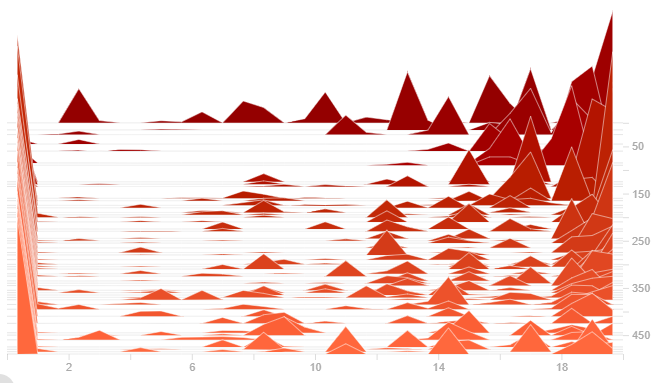
\includegraphics[width=1.0\textwidth]{figures/5_evaluation_figs/algo_training_fig/dqn_auction_prices.png}
%        \caption{Deep Q Network auction prices}
%        \label{fig:dqn-auction-prices}
%    \end{minipage}\hfill
%    \begin{minipage}{0.5\textwidth}
%        \centering
%        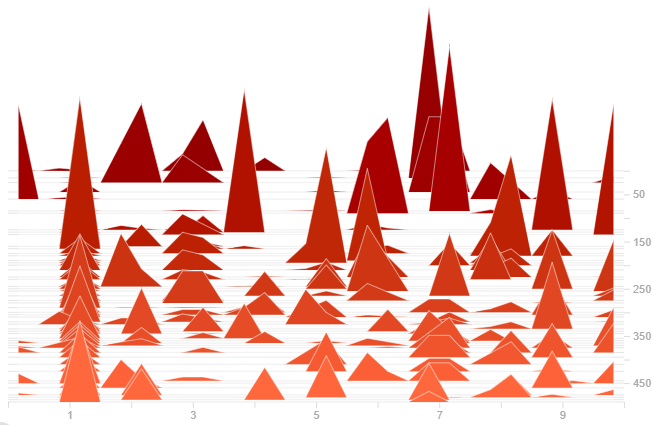
\includegraphics[width=1.0\textwidth]{figures/5_evaluation_figs/algo_training_fig/dqn_weightings.png}
%        \caption{Deep Q Network resource weightings}
%        \label{fig:dqn-resource-weightings}
%    \end{minipage}
%\end{figure}

\subsection{Environment and Agent number training}
\label{subsec:environment-and-agent-number-training}
The analysis of the different Reinforcement Learning algorithms and neural network architectures in
Subsection~\ref{subsec:reinforcement-learning-algorithm-training} and~\ref{subsec:neural-network-architecture-training}
respectively assume two qualities that this subsection analyses. These are that the training and evaluation environments
used and the number of agents used during training.

As there are huge ranges of possible environment settings that agents could be trained, investigating agent environment
generality is a challenge and an important measure within machine learning. This is of particular importance for this
work, as in real-life, the environment that agents experiences can be unpredictable and different from those
trained on. This means that agents should learn to generalise and not overfit to particular environments used during
training.

The other assume quality is due an advantage of the Vickrey auction over alternative auctions, explored in
Section~\ref{sec:auctioning-of-tasks}, that is it's Incentive Compatibility. This auction property means that the
dominant strategy for all agents is to bid truthfully, that is the agent's true evaluation of the task. Therefore due
to agents not needing to learn to "out bid" each other, this allows for the possibility to learn through self-play.

\begin{wrapfigure}{r}{0.3\textwidth}
    \includegraphics[width=0.3\textwidth]{figures/5_evaluation_figs/env_agent_num_training_fig/legend.png}
    \caption{Environment and number of Agents Legend}
    \label{fig:env-training-legend}
\end{wrapfigure}

Therefore this subsection compare the results of agents that are trained on a single environment setting and those
trained on multiple environment settings and when multiple or single agents are trained together. These are compared
using a set of pre-generated environments, 5 from the single environment setting and 20 from the multiple
environment settings to evaluate agents.

\begin{figure}[H]
    \centering
    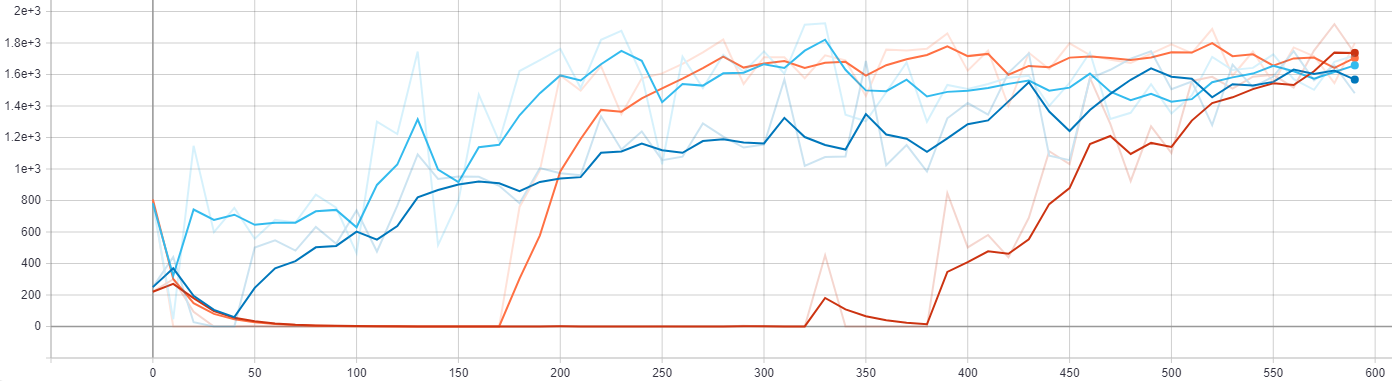
\includegraphics[width=\linewidth]{figures/5_evaluation_figs/env_agent_num_training_fig/num_completed_tasks.png}
    \caption{Environment and number of Agents - Number of completed tasks (Multi-env settings)}
    \label{fig:env_num_completed_tasks}
\end{figure}

\begin{figure}[H]
    \centering
    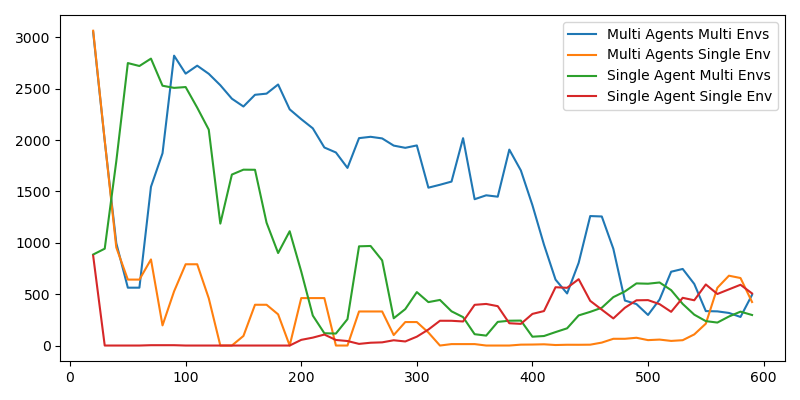
\includegraphics[width=\linewidth]{figures/5_evaluation_figs/env_agent_num_training_fig/num_failed_tasks.png}
    \caption{Environment and number of Agents - Number of failed tasks (Multi-env settings)}
    \label{fig:env_num_failed_tasks}
\end{figure}

\begin{figure}[H]
    \centering
    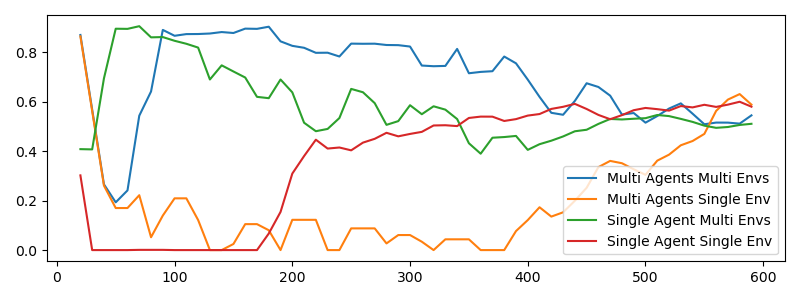
\includegraphics[width=\linewidth]{figures/5_evaluation_figs/env_agent_num_training_fig/percent_tasks.png}
    \caption{Environment and number of Agents - Percentage of tasks attempted (Multi-env settings)}
    \label{fig:env_percent_tasks}
\end{figure}

\begin{figure}[H]
    \centering
    \begin{minipage}{0.75\linewidth}
        \centering
        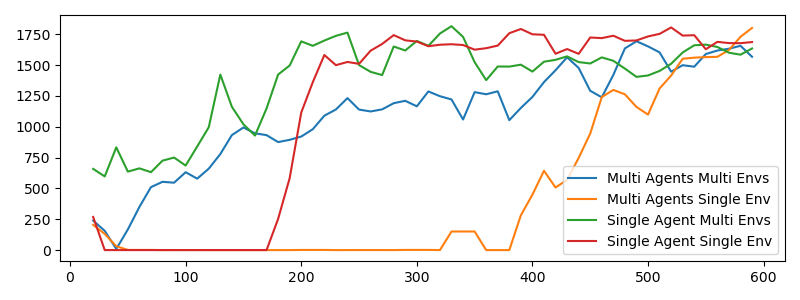
\includegraphics[width=\linewidth]{figures/5_evaluation_figs/env_agent_num_training_fig/single_env_num_completed_tasks.png}
        \caption{Environment and number of Agents - Number of completed tasks (Single env settings)}
        \label{fig:single_env_num_completed_tasks}
    \end{minipage}\hfill
    \begin{minipage}{0.25\linewidth}
        \centering
        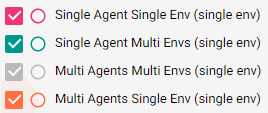
\includegraphics[width=\linewidth]{figures/5_evaluation_figs/env_agent_num_training_fig/single_env_legend.png}
        \caption{Single environment results legend}
        \label{fig:single_env_legend}
    \end{minipage}
\end{figure}

Figure~\ref{fig:env_num_completed_tasks} shows that for the agents trained using only a single environment, took
over 150 episodes for the single agent and 350 episodes for the multiple agents to achieve over 25\% of the final total
tasks allocated. This is in comparison to both the single and multiple agents that were trained with multiple
environments that were able to achieve better results faster than the single environment agents. \\
Surprisingly, the number of tasks allocated by all agents after 600 episodes are within 6\% of each other. This being
despite the single environment agents not being trained on the multi-environment settings that it is being evaluated on.
This means agents are able to generalised efficiently to unknown environments however this is difficult to confirm in
real-life due to the multi-environment trained are only a small subset of the possible environment will experience in
real-life.

The agents were simultaneously evaluated on the single environment setting with the single environment agents
achieving 10\% higher than the multiple environment agents. This is understandable due to single environment being
more "specialised" in the single environment allowing the agent to maximise profit compared to the multi-environment
agent that have learnt to maximise profit over more environments.

\subsection{Reinforcement learning algorithm training}
\label{subsec:reinforcement-learning-algorithm-training}

\begin{wrapfigure}{r}{0.2\textwidth}
    \includegraphics[width=0.2\textwidth]{figures/5_evaluation_figs/algo_training_fig/legend.png}
    \caption{Reinforcement learning algorithm Legend}
    \label{fig:algo-training-legend}
\end{wrapfigure}

In table~\ref{tab:reinforcement_learning_algorithms}, a range of reinforcement learning algorithms implemented,
to compare the effectiveness of the algorithms, each were trained. This was done using three task pricing agents with
a single resource weighting on multiple environment settings for training due the reasoning given in
Subsection~\ref{subsec:environment-and-agent-number-training}. Due to time limits, the policy gradients agents were
only trained for 24 hours however during this time were only about to complete 300 to 400 episodes of training while
the Dqn agents were able to train in 15 hours for 600 episodes.

\begin{figure}[H]
    \centering
    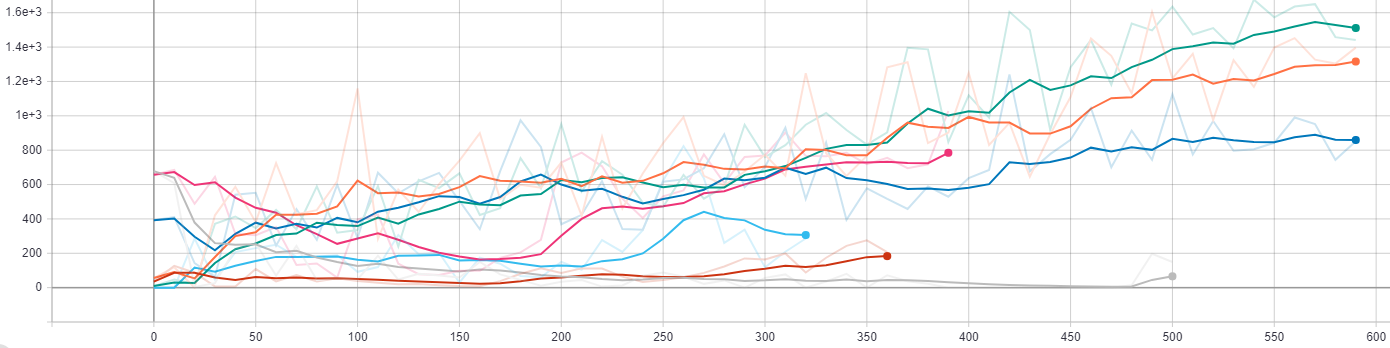
\includegraphics[width=\linewidth]{figures/5_evaluation_figs/algo_training_fig/num_completed_tasks.PNG}
    \caption{Reinforcement learning algorithms - Number of completed tasks}
    \label{fig:algo_num_completed_tasks}
\end{figure}

\begin{figure}[H]
    \centering
    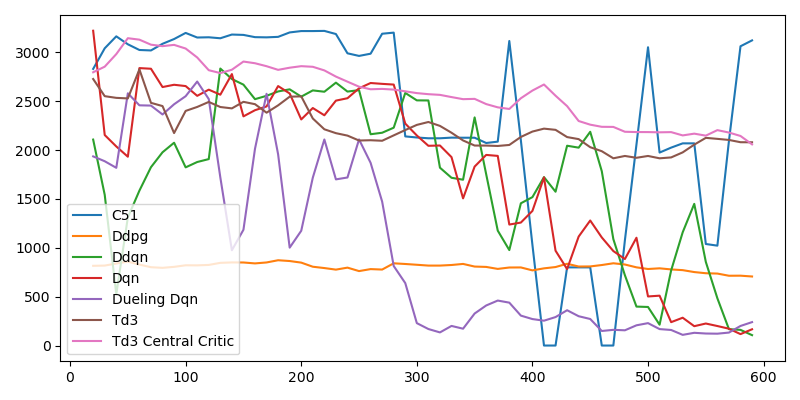
\includegraphics[width=\linewidth]{figures/5_evaluation_figs/algo_training_fig/num_failed_tasks.png}
    \caption{Reinforcement learning algorithms - Number of failed tasks}
    \label{fig:algo_num_failed_tasks}
\end{figure}

\begin{figure}[H]
    \centering
    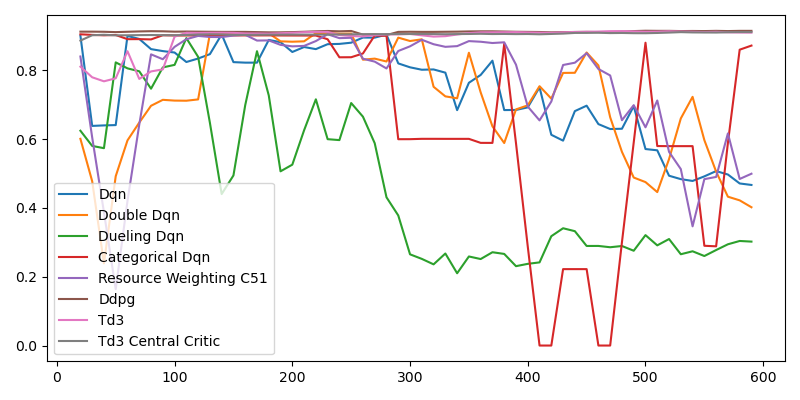
\includegraphics[width=\linewidth]{figures/5_evaluation_figs/algo_training_fig/percent_tasks.png}
    \caption{Reinforcement learning algorithms - Percentage of tasks attempted}
    \label{fig:algo_percent_tasks}
\end{figure}

The results did not match expectation due to the heuristic Dqn agents (Double Dqn and Dueling Dqn) achieved a fewer
number of completed tasks (figure~\ref{fig:algo_num_completed_tasks}) than the simpler Dqn agents despite no changes
being made to the agents except to the heuristic modifications. Another surprise were how badly the Ddpg agents did
in comparison to the Dqn agents, particularly with regards to the percentage of tasks attempted
(figure~\ref{fig:algo_percent_tasks}) where it appears that Ddpg agents attempted every task resulting in the agents
being unable successfully complete as many tasks. However the Td3 Central critic (where the critic was the same network
shared by all task pricing agents) did achieve results that are on par with the Dqn agent but due to training time
limits this can't be known if this relationship will continue. The Categorical Dqn agent implemented, while could
completed much simpler reinforcement learning problem, the agent struggles with the environment however this problem
is believed to be a problem with the implementation rather than the algorithm not being effective.

\subsection{Neural network architecture training}
\label{subsec:neural-network-architecture-training}
\begin{wrapfigure}{r}{0.25\textwidth}
    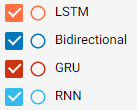
\includegraphics[width=0.25\textwidth]{figures/5_evaluation_figs/net_arch_training_fig/legend.png}
    \caption{Network architecture legend}
    \label{fig:net-arch-training-legend}
\end{wrapfigure}

There are a wide-range of compatible neural network architectures that agents can use, as outlined in
table~\ref{tab:neural_network_layers}. To compare these architectures, four different network architectures are trained:
RNN~\citep{RNN}, LSTM~\citep{LSTM}, GRU~\citep{GRU} and Bidirectional~\citep{Bidirectional} using an LSTM network.
These networks are trained using the DQN algorithm due to it constant performance compared to the DDPG agents that can
get stuck in a local maxima making the results probably inconstant as shown in the previous section. A Seq2Seq agent
was also implemented as an experimental agent with a LSTM Dqn Agent for the task pricing agent and the Seq2Seq Policy
Gradient agent acting only for the resource weighting. \\

\begin{figure}[H]
    \centering
    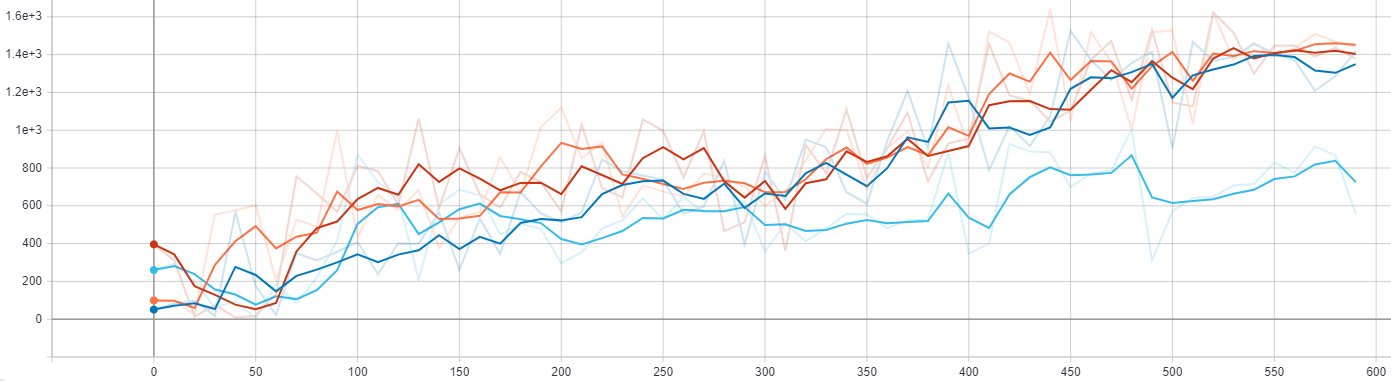
\includegraphics[width=\linewidth]{figures/5_evaluation_figs/net_arch_training_fig/num_completed_tasks.PNG}
    \caption{Network Architecture - Number of completed tasks}
    \label{fig:net_arch_num_completed_tasks}
\end{figure}

\begin{figure}[H]
    \centering
    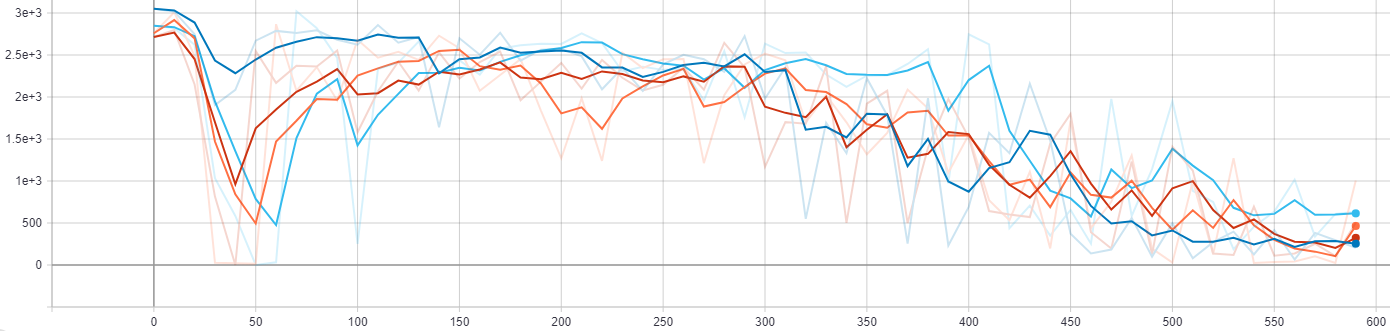
\includegraphics[width=\linewidth]{figures/5_evaluation_figs/net_arch_training_fig/num_failed_tasks.png}
    \caption{Network Architecture - Number of failed tasks}
    \label{fig:net_arch_num_failed_tasks}
\end{figure}

\begin{figure}[H]
    \centering
    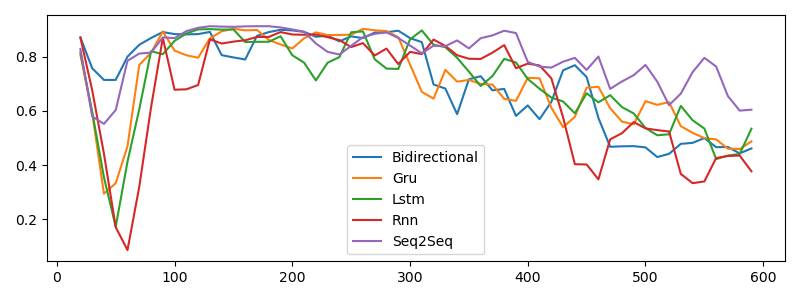
\includegraphics[width=\linewidth]{figures/5_evaluation_figs/net_arch_training_fig/percent_tasks.png}
    \caption{Network Architecture - Percent of tasks attempted}
    \label{fig:net_arch_percent_tasks}
\end{figure}

As shown in figure~\ref{fig:net_arch_num_completed_tasks}, the LSTM, GRU and Bidirectional networks all achieved a
similar score in the number of tasks completed while the RNN network achieves 30\% less. This is understandable due to
the known of problem for RNNs of vanishing or exploding gradients as explained in Table~\ref{tab:neural_network_layers}.
The Bidirectional neural network doesn't achieve a greater score that the other networks despite the network
architecture allowing all inputs to be passed in is understandable due to the network providing a single output.
Because of this, all tasks to the network are considered before any action is taken which is why the Bidirectional
network didn't achieve a better score. However the Bidirectional seems more resilient to changes during training as
shown in figure~\ref{fig:net_arch_num_failed_tasks} and~\ref{fig:net_arch_percent_tasks}. At episode 30 to 70, all
of the network's (except Bidirectional), the number of failed tasks and number of attempted tasks suddenly drop, most
likely to an over evaluating to not bid on any tasks by the task pricing agents.
